\documentclass{beamer}

\usepackage{tikz}
\usepackage[style=authortitle,backend=bibtex]{biblatex}
\addbibresource{presentation.bib}

\mode<presentation>{
	\usetheme{Madrid}
	\usecolortheme{whale}
	\setbeamercovered{transparent}
}

\title[FS Implementation]{{\small CS270: Advanced Operating Systems}\\Course Project on File System Implementation}
\author[THE Team]{Gareth George \and Thomas Schibler \and Nazmus Saquib}
\institute[CS grads, UCSB]{Graduate Students\\
Department of Computer Science\\
University of California Santa Barbara}
\titlegraphic{
\includegraphics[width=0.2\textwidth]{ucsb-logo.png}}

\AtBeginSection[]
{
  \begin{frame}<beamer>
    \frametitle{Outline}
    \tableofcontents[currentsection]
  \end{frame}
}

\begin{document}
\newcommand{\continued}{\textit{(Cntd.)}}
\newcommand\pro{\item[$+$]}
\newcommand\con{\item[$-$]}
%titlepage
\begin{frame}
\titlepage
\end{frame}

% introduce members
% what is the architecture of the solution
% basics/beyond basics: what things did you try to figure out
% what challenges
% what new things
% what part of the project led us to think in an unusual way about OS
\section{Introduction}

\begin{frame}
\frametitle{Introduction}
	Design goals:\\[0.5em]
	\begin{itemize}[<+->]
	\setlength\itemsep{1em}
	\item High reliability
	\item Simplicity
	\item Memory mapped files
		\begin{itemize}
			\item performance gain at the cost of reliability
			\item acceptable for high performance system
			\item can be seen in Mach
		\end{itemize}
	\item General data structures
	\item Log structured file system (LFS)
\end{itemize}
\end{frame}

\begin{frame}
	\frametitle{Introduction: Memory Mapped Files}
	\begin{itemize}[<+->]
		\setlength\itemsep{1em}
		\pro Efficient paging as kernel handles it
		\con Lesser direct control
		\con Restricts fine-grained control over writes
	\end{itemize}
\end{frame}

\section{Architecture}
\begin{frame}
	\frametitle{Architecture: Hybrid Log Structured File System (LFS)}
	\begin{itemize}[<+->]
		\setlength\itemsep{1em}
		\item Superblock
			\begin{itemize}
				\item holds references to all other file system data structures
				\item initializes 
					\begin{itemize}
						\item the inode table 
						\item the segment controller
					\end{itemize}
			\end{itemize}
		\item Inodes
			\begin{itemize}
				\item closely resembles inodes from ``A Fast File System for UNIX''
				\item each inode contains 8 direct, 1 indirect, 1 double indirect, and 1 triple indirect blocks
				\item additionally complicated by the need for an algorithm that allows moving both data blocks and indirect pages belonging to an inode
			\end{itemize}
	\end{itemize}
\end{frame}



\section{Beyond Basics}
\begin{frame}
\frametitle{Beyond Basics}
\end{frame}

\section{Challenges}

\begin{frame}
\frametitle{Challenges}
\begin{itemize}[<+->]
	\setlength\itemsep{1em}
	\item Memory mapped interface
	\item Dropped pointer
	\item Off by one
\end{itemize}

\begin{center}
\onslide<4-5>{\tikz\node[draw, align=center,minimum width=12cm,minimum height=1cm,fill=blue!20]{Language choice: C++ 11};}
\end{center}
\begin{itemize}[<+->]
	\setlength\itemsep{1em}
	\pro proper exception handling
	\pro proper memory management
\end{itemize}
\end{frame}

\section{Performance Benchmark}

\begin{frame}
\frametitle{Performance Benchmark}
	%\begin{itemize}
	%\setlength\itemsep{1em}
	%\item Synchronous memory mapped
	%\item Asynchronous memory mapped
	%\item Non-memory mapped
	%\end{itemize}
	\begin{figure}
		\centering
		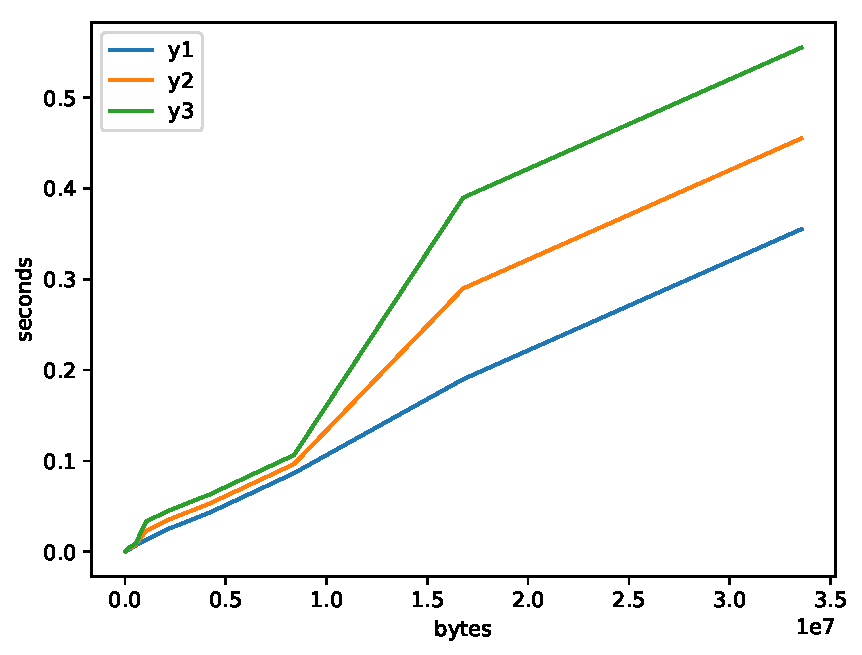
\includegraphics[width=0.85\textwidth]{fig.pdf}
	\end{figure}
\end{frame}

\section{Conclusion}
\begin{frame}
\frametitle{Conclusion}
\end{frame}

\section{Questions}
\begin{frame}
	\begin{center}
		{\fontsize{20}{20}\selectfont
			\textbf{Questions?}
		}
	\end{center}
\end{frame}


\end{document}
